% fluxograma_animatronico_refinado.tex
\documentclass[border=10pt]{standalone}
\usepackage{tikz}
\usetikzlibrary{shapes.geometric, arrows.meta, positioning}

\begin{document}
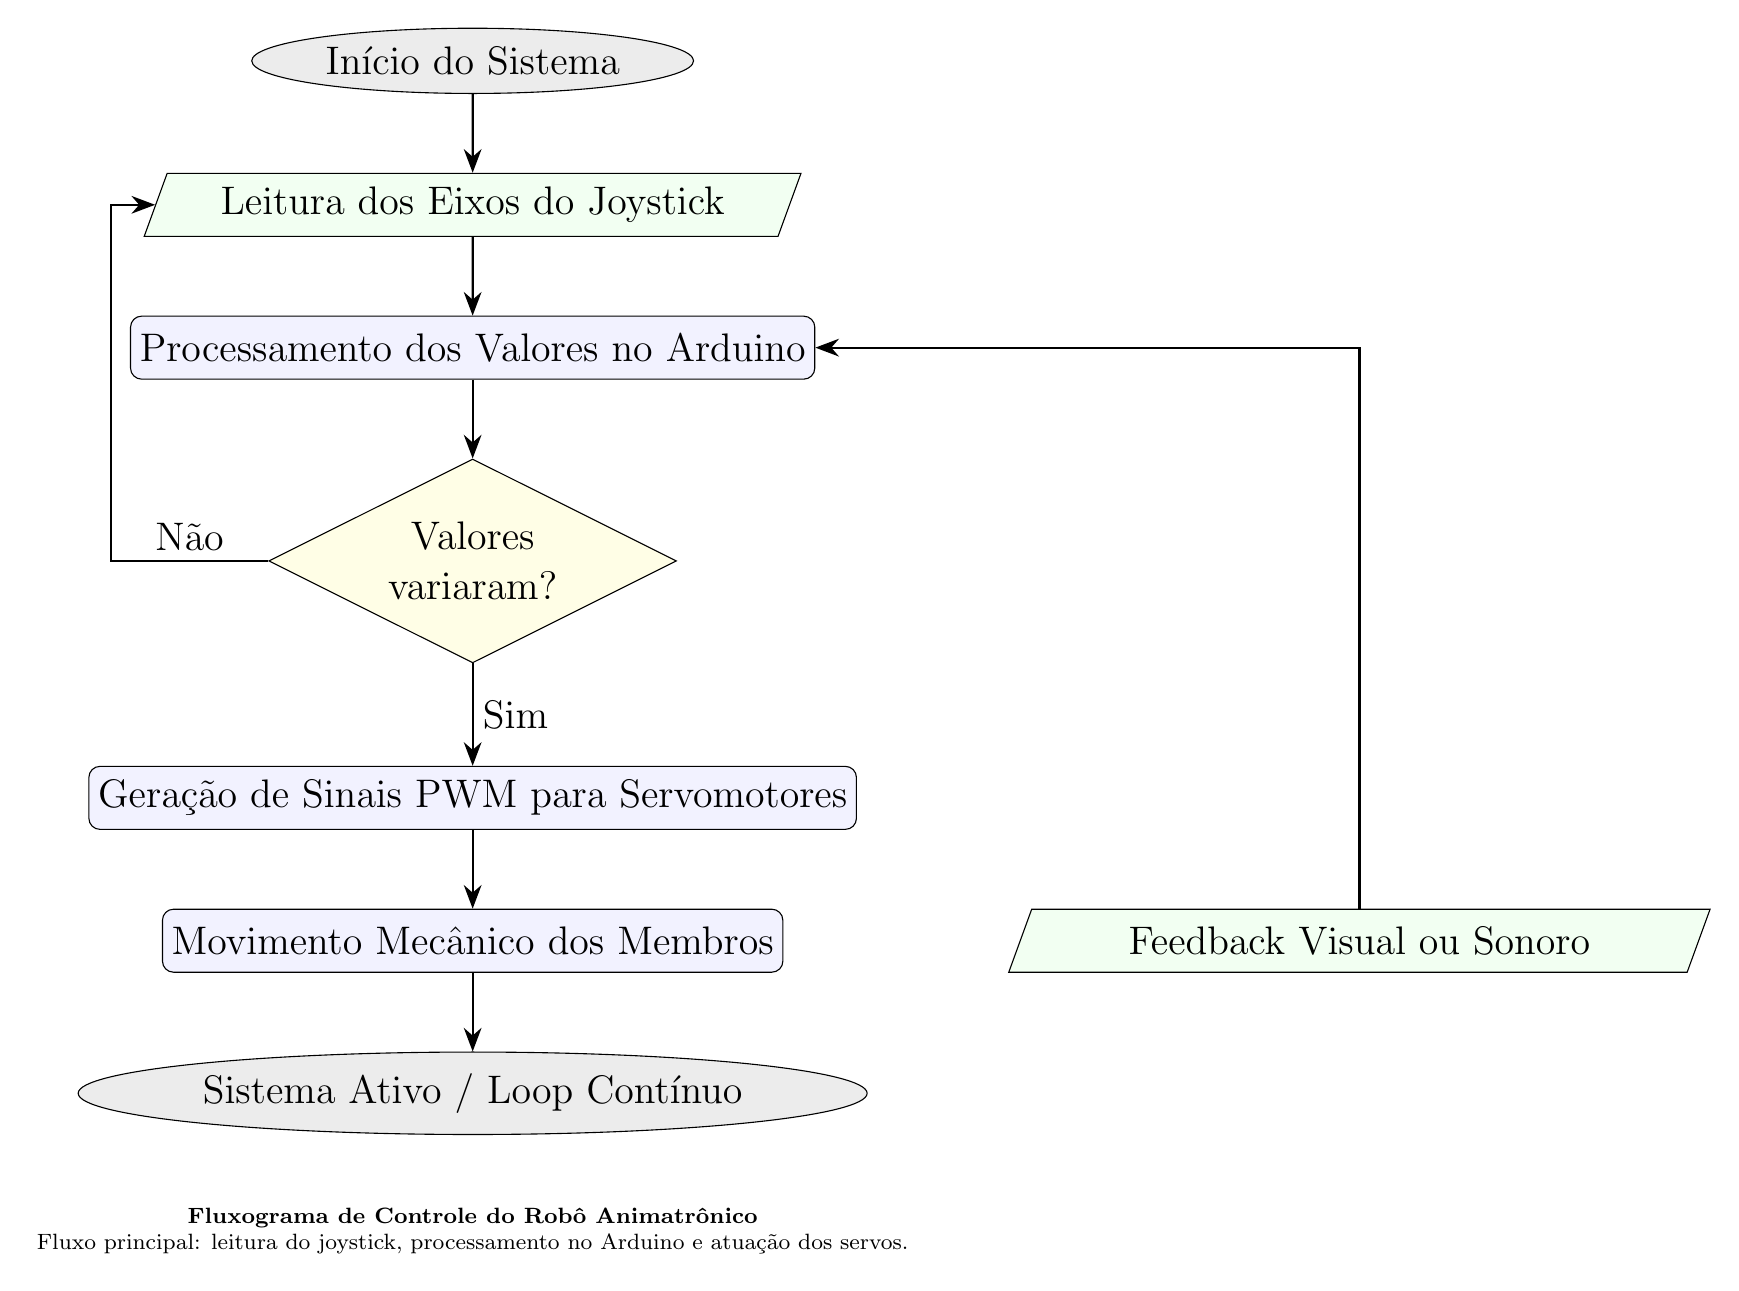
\begin{tikzpicture}[
  node distance=10mm and 22mm,
  font=\Large,
  startstop/.style={ellipse, draw, fill=gray!15, minimum width=25mm, minimum height=8mm, align=center},
  process/.style={rectangle, draw, fill=blue!5, rounded corners, minimum width=35mm, minimum height=8mm, align=center},
  decision/.style={diamond, aspect=2, draw, fill=yellow!10, align=center, text width=30mm, inner sep=1pt},
  io/.style={trapezium, trapezium left angle=70, trapezium right angle=110, draw, fill=green!5, minimum width=35mm, minimum height=8mm, align=center},
  arrow/.style={-{Stealth[length=3mm]}, thick}
]

% NODES
\node[startstop] (inicio) {Início do Sistema};
\node[io, below=of inicio] (joystick) {Leitura dos Eixos do Joystick};
\node[process, below=of joystick] (processa) {Processamento dos Valores no Arduino};
\node[decision, below=of processa] (decide) {Valores variaram?};
\node[process, below=of decide, yshift=-3mm] (servo) {Geração de Sinais PWM para Servomotores};
\node[process, below=of servo] (mov) {Movimento Mecânico dos Membros};
\node[io, right=30mm of mov] (feedback) {Feedback Visual ou Sonoro};
\node[startstop, below=of mov] (fim) {Sistema Ativo / Loop Contínuo};

% FLOW
\draw[arrow] (inicio) -- (joystick);
\draw[arrow] (joystick) -- (processa);
\draw[arrow] (processa) -- (decide);
\draw[arrow] (decide) -- node[right]{Sim} (servo);
\draw[arrow] (servo) -- (mov);
\draw[arrow] (mov) -- (fim);
\draw[arrow] (feedback) |- (processa);
\draw[arrow] (decide.west) -- ++(-20mm,0) node[midway, above]{Não} |- (joystick.west);

% ANOTAÇÃO
\node[align=center, below=8mm of fim, font=\footnotesize] {
\textbf{Fluxograma de Controle do Robô Animatrônico}\\
Fluxo principal: leitura do joystick, processamento no Arduino e atuação dos servos.
};

\end{tikzpicture}
\end{document}

